%% Discover Artificial Intelligence (Springer Nature) manuscript, English version of the Japanese draft ver4
%% (paper/ja_v4/, 2026-11-17; structure of Mensh & Kording 2017 and MIT CommLab). Class: sn-jnl (copied once from the Springer Nature template on 2026-11-14).
%% Numbers are copied from the checked Japanese draft (each section of ja_v2 lists its sources in comments).
\documentclass[sn-nature,pdflatex]{sn-jnl}

\usepackage{amsmath,amssymb,amsfonts}
\usepackage{graphicx}
\usepackage{booktabs}
\usepackage{multirow}
\usepackage{xcolor}
\usepackage{array}
\usepackage{placeins}

% Draft markers (remove before submission).
\newcommand{\TBA}{\textcolor{red}{TBA}}
\newcommand{\PROV}[1]{\textcolor{orange}{#1}}  % value not yet re-checked
\newcommand{\pt}{\,points}

\begin{document}

\title[Other modalities make up for missing labels]{Other modalities make up for missing labels: emotion-wise weighted pseudo-labels for multimodal emotion recognition on a new corpus with few labels}

\author*[1]{\fnm{TODO} \sur{TODO}}\email{TODO}

\affil*[1]{\orgdiv{TODO}, \orgname{TODO}, \orgaddress{\city{TODO}, \country{Japan}}}

\abstract{Multimodal emotion recognition (MER) classifiers have been reported to degrade on unseen corpora, and labelling a new corpus is costly because each utterance needs several raters. Domain adaptation and semi-supervised methods use same-modality unlabelled data, whereas in MER unlabelled utterances also have other modalities whose predictions can serve as pseudo-labels; to our knowledge, which helps more with a few labels per emotion has not been compared. With linear classifiers on frozen audio, visual and text encoders, we show that retraining audio classifiers on pseudo-labels including other modalities gave higher unweighted average recall (UAR) than 11 domain adaptation, semi-supervised and test-time adaptation methods, and that UAR was higher the more accurate the pseudo-labels were. With the error split into a bias towards some emotions and the remaining error, these pseudo-labels reduced the latter in far more conditions than same-modality unlabelled utterances. As the modality that best separated each emotion varied by corpus, we propose late fusion that weights each modality per emotion using the few labels and other corpora, for more accurate pseudo-labels. On AFEW, IEMOCAP, MOSEI and MELD, also used to design it, its fused predictions were more accurate than equal-weight fusion in 11 of 12 conditions (5, 10, 25 labels per emotion), and early-fusion classifiers retrained on its pseudo-labels outperformed those retrained on equal-weight ones in 11 of 12. Audio classifiers retrained on multimodal pseudo-labels alone outperformed those retrained on 5 or 10 labels per emotion, so the other modalities made up for part of the missing labels.}

\keywords{Multimodal emotion recognition, Cross-corpus transfer, Semi-supervised domain adaptation, Few labels, Pseudo-labels, Distillation, Late fusion}

\maketitle

% English version of paper/ja_v4/01_序論.md (ver4, 2026-11-17). MIT CommLab introduction formula: general background -> specific background -> knowledge gap -> "here we show". No section roadmap (Peyton Jones). Sentences carried over from v3_01_introduction.tex keep their checked wording; changed sentences follow reviews/v4_ja/citations_2026-11-17.md.
\section{Introduction}\label{sec:intro}

Multimodal emotion recognition (MER) estimates a speaker's emotion from the voice, face and words of the same utterance. Emotion corpora differ in environmental noise, recording devices, acted versus natural elicitation and speaker demographics \cite{gideon2021addog}, and also in how they were annotated. Emotion classifiers trained on one corpus have been reported to perform worse on other corpora \cite{ryumina2025,gideon2021addog}. Using MER on a new corpus not used for training (hereafter the target) therefore requires adapting the classifiers to it. Labels of naturally expressed emotions, however, are collected from several raters who watch or listen to each utterance, which is costly to repeat for every new corpus \cite{parthasarathy2020ladder,abdelwahab2018dann}. We consider a target with only a few labels per emotion.

Standard methods that adapt classifiers to a target with few labels use data of the same modality as the classifier. Domain adaptation uses labelled utterances of other corpora (hereafter sources) and unlabelled target utterances \cite{ganin2016dann,sun2016coral}, and semi-supervised domain adaptation adds a few target labels \cite{saito2019mme}. In emotion recognition, adapting classifiers with sources and unlabelled target utterances or a few target labels has been studied mainly for audio classifiers \cite{abdelwahab2018dann,gideon2021addog,feng2023}. In MER, by contrast, unlabelled utterances also come with voice, face and words, so the classifier of one modality can be trained towards the predictions of classifiers of other modalities. Albanie et al.\ \cite{albanie2018} attached the predictions of a facial classifier to unlabelled videos and trained an audio emotion classifier towards them, and Zhang et al.\ \cite{zhang2021combining} combined training towards targets that include predictions of other modalities with semi-supervised learning. We call the four-emotion probabilities that classifiers including other modalities assign to unlabelled utterances \emph{pseudo-labels}, and retraining a classifier towards them without temperature \emph{distillation} \cite{hinton2015distilling,albanie2018}.

However, whether same-modality methods using unlabelled utterances or pseudo-labels including other modalities make better classifiers in cross-corpus MER with only a few target labels per emotion has not been compared under the same conditions. Albanie et al.\ and Zhang et al.\ did not evaluate this setting, and training on the predictions of a more accurate model of another modality has been reported not to always improve the trained model \cite{xue2023mfh}. Audio and visual classifiers have also been reported to recognise different emotions well within one corpus \cite{busso2004}, but how the predictions of the audio, visual and text classifiers should be combined into pseudo-labels is unknown.

With each of AFEW, IEMOCAP, MOSEI and MELD in turn as the target, we compare distillation on pseudo-labels including other modalities with 11 domain adaptation, semi-supervised and test-time adaptation methods that do not use such pseudo-labels, under the same conditions. The classifiers are linear classifiers on features of frozen pretrained audio, visual and text encoders; this is a setting for measuring what makes the classifiers better, not a proposed architecture, and we do not claim that the results hold for fine-tuned encoders (Sect.~\ref{sec:limitations}). The unweighted average recall (UAR, the mean of per-emotion recalls) of audio classifiers retrained by distillation was higher than that of the 11 methods, and across classifiers retrained on pseudo-labels from different providers, UAR was higher the more accurate the pseudo-labels were relative to the classifier before retraining. In addition, to make the pseudo-labels more accurate, we propose late fusion that sets per-emotion weights of each modality's predictions from the few target labels and the source corpora (Fig.~\ref{fig:overview}). The fused predictions of the proposal had higher UAR than predictions fused with equal weights in 11 of 12 conditions (four target corpora with 5, 10 and 25 labels per emotion), and classifiers retrained on the proposal's pseudo-labels had higher UAR than those retrained on the equal-weight pseudo-labels in 11 of 12 conditions.

\begin{figure}[t]
\centering
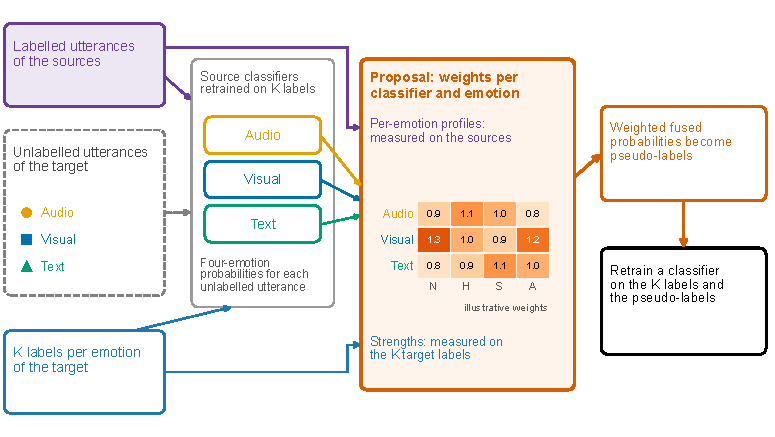
\includegraphics[width=\textwidth]{figures/fig_v4_overview_en.pdf}
\caption{The proposal combines the probabilities that the audio, visual and text classifiers (started from the source classifiers and retrained on the K target labels per emotion; Sect.~\ref{sec:distill}) assign to unlabelled target utterances with one weight per classifier and emotion, turns the fused probabilities into pseudo-labels, and retrains a classifier on them and the K labels per emotion. Each weight is built from the classifier's strength (its mean reliability over the four emotions), measured on the K target labels, and its per-emotion profile (how much its reliability for each emotion deviates from that mean), measured on the labelled source corpora. Weight values are illustrative}\label{fig:overview}
\end{figure}

% English version of paper/ja_v4/02_関連研究.md (ver4, 2026-11-17): three paragraphs, each closing with the difference from this study. Cited claims carried over from v3_02_related.tex; the regrouped sentences follow reviews/v4_ja/citations_2026-11-17.md.
\section{Related work}\label{sec:related}

\subsection{Adapting classifiers to a target with few labels}\label{sec:rel-da}
Learning representations that do not reveal the domain (domain-adversarial neural networks, DANN) \cite{ganin2016dann} and aligning feature covariances (CORAL) \cite{sun2016coral} have been proposed for unlabelled targets, entropy minimisation and pseudo-labels for semi-supervised learning without domain shift \cite{grandvalet2004,lee2013pseudolabel}, and minimax entropy (MME) for semi-supervised domain adaptation, in which the target has a few labels \cite{saito2019mme}. Adding source data can also lower target performance (negative transfer) \cite{wang2019negative}. In emotion recognition, adversarial learning that aligns representations with unlabelled target utterances \cite{abdelwahab2018dann} and learning that pulls together representations learned per corpus \cite{gideon2021addog} have been proposed for audio classifiers; for targets with a few labels, Feng and Chaspari \cite{feng2023} proposed metric learning for audio features, Li et al.\ \cite{li2021acted} adaptation of audio and video between acted and improvised speech, and He et al.\ \cite{he2025m4ser} a method using audio and speech-recognition transcripts. These domain adaptation and semi-supervised methods, and the adaptation methods for emotion recognition, all adapt the classifier with data of the same modality as the classifier being retrained. MER fusion methods, including those for sentiment polarity, have instead been evaluated by training and testing within one corpus \cite{zadeh2017tfn,mittal2020m3er,yu2021selfmm,yun2024telme}, and the cross-corpus evaluations of Ryumina et al.\ \cite{ryumina2025} and Lian et al.\ \cite{lian2026merbench} did not use target labels. We compare 11 methods, including DANN, CORAL, entropy minimisation, self-training and MME (Sect.~\ref{sec:distill}), with pseudo-labels including other modalities under the same conditions.

\subsection{Learning from predictions of other modalities}\label{sec:rel-distill}
Albanie et al.\ \cite{albanie2018} attached facial-expression predictions to unlabelled videos and trained an audio emotion classifier on them, and Zhang et al.\ \cite{zhang2021combining} combined training towards targets that include predictions of other modalities with semi-supervised learning. Transferring representations or predictions of one modality to a model of another through paired unlabelled data is also used outside emotion recognition \cite{gupta2016,jaritz2020xmuda}. Training on the predictions of a more accurate model of another modality has been reported not to always improve the trained model \cite{xue2023mfh}. Three comparisons are close to ours. Zhang et al.\ (2021) compared pseudo-labels including facial predictions with same-modality semi-supervised learning for speech emotion recognition, but used all training labels of the evaluated corpus (IEMOCAP) and did not compare domain adaptation methods. Jaritz et al.\ \cite{jaritz2023xmossda} compared cross-modal learning with uni-modal unsupervised domain adaptation methods moved to a semi-supervised setting, but for 3D semantic segmentation. Zhang et al.\ (2024) \cite{zhang2024amanda} proposed a multimodal domain adaptation method that uses no target labels between IEMOCAP, MELD, MOSEI and MSP-IMPROV and compared it with DANN and other methods, but not with distillation on pseudo-labels from other modalities. To the best of our knowledge, no prior study has compared, in cross-corpus MER with audio, visual and text and only a few target labels per emotion, distillation on pseudo-labels including other modalities with 11 domain adaptation, semi-supervised and test-time adaptation methods that do not use such pseudo-labels (versions moved to linear classifiers on frozen features) under the same conditions.

\subsection{Late fusion and reliability weights}\label{sec:rel-fusion}
Zadeh et al.\ \cite{zadeh2017tfn} criticised late fusion, which trains unimodal classifiers separately and combines their predictions, for not learning interactions between modalities because it assumes that simple weighted averaging is a proper fusion approach. Predictions can be combined by product or sum rules \cite{kittler1998}. Busso et al.\ \cite{busso2004} reported that modality strengths differ by emotion. Kaya et al.\ \cite{kaya2017} chose model-by-emotion weights on AFEW by random search on validation data, M3ER \cite{mittal2020m3er} learned a multiplicative fusion layer that strengthens reliable modality cues per utterance, and Mar\'in et al.\ \cite{marin2026classwise} used per-utterance, per-emotion modality weights output by a network trained with all labels within one corpus. Kaya et al.\ determined the weights, and M3ER and Mar\'in et al.\ the layers that output them, with labelled data of the evaluated corpus. With few training samples, a model trained on more modalities has also been argued to be able to fall below a model trained on a subset of them \cite{huang2021}. Like Kaya et al., the proposal uses one weight per classifier and emotion, but it sets the weights from a few target labels and the source corpora. We found no study that splits the weights into classifier strengths measured on a few target labels per emotion and per-emotion profiles measured on the source corpora.

% English version of paper/ja_v4/03_方法.md (ver4, 2026-11-17). The table of compared methods was removed at the researcher's request; the methods are listed in the text. Conditions are called by name (the code list (A0)--(E2) is Table S7). All procedure-order disclosures are gathered in Sect. 3.7 (Mensh & Kording rule 3). Sentences are carried over from v3_03_setup, v3_04_analysis (4.1, 4.2, 4.4), v3_05_method and v3_06_experiments where the Japanese text was carried over.
\FloatBarrier
\section{Methods}\label{sec:methods}

\subsection{Corpora and settings}\label{sec:setup}
We use six corpora that differ in elicitation, recording and annotation as seven groups (Table~\ref{tab:corpora}). IEMOCAP \cite{busso2008iemocap} is split into improvised and scripted groups, because in scripted sessions ten actors read the same lines and a text classifier could succeed by memorising them. Labels are mapped to the four emotions present in all seven groups, Neutral, Happy, Sad and Angry (the four emotions of Ryumina et al.\ \cite{ryumina2025}), and utterances with other labels are not used. IEMOCAP uses the plurality label of the raters, with neutral as Neutral, happy and excited as Happy, sad as Sad and angry as Angry; frustration is not mapped to Angry, and disgust, fear, surprise, other and utterances without a plurality are not used. MELD uses neutral, joy, sadness and anger, and AFEW and CREMA-D the labels corresponding to Neutral, Happy, Sad and Angry; disgust, fear and surprise are not used (CREMA-D has no surprise). RAVDESS uses neutral, happy, sad and angry; calm is not merged into Neutral, and calm, fearful, disgust and surprised are not used. In MOSEI, an utterance with exactly one emotion of intensity at least 0.5 receives that emotion, one with none receives Neutral, and one with two or more is not used, so MOSEI Neutral is not a neutral rating by annotators.

\begin{table}[t]
\caption{The seven groups. Elicitation, recording and annotation follow the original papers. Speaker and utterance counts are after restricting to four emotions, for the all-source setting (and the single-source setting of Supplementary Information S2); utterance and per-emotion counts are for the audio (WavLM) set, with differing visual or text counts in parentheses. The last column gives, for the LOCO setting (utterances with audio, visual and text; CREMA-D: audio and visual), the utterances, the clusters used to form test folds and their effective number $(\sum_g n_g)^2/\sum_g n_g^2$ for cluster sizes $n_g$; per-emotion LOCO counts are in Table~S1. Mod.: modalities. All corpora are in English (RAVDESS: North American English)}\label{tab:corpora}
\footnotesize\setlength{\tabcolsep}{3pt}
\begin{tabular}{@{}p{1.55cm}p{1.7cm}p{1.95cm}p{0.75cm}r p{1.5cm}p{1.7cm}p{1.35cm}@{}}
\toprule
Group & Elicitation, recording & Annotation & Mod. & Speakers & Utterances & N / H / S / A & LOCO (clusters, effective) \\
\midrule
AFEW \cite{dhall2012afew,dhall2013emotiw} & Movie acting (partly natural); scenes found by subtitle emotion words & Facial-expression category by raters & A, V, T$^{b}$ & 282$^{a}$ & 795 & 207 / 213 / 178 / 197 & 790 (51, 14.99) \\
IEMOCAP impro.\ \cite{busso2008iemocap} & Improvised acting; dyadic lab sessions & Plurality of raters' categories & A, V, T & 10 & 2,943 & 1,099 / 947 / 608 / 289 & 2,943 (5, 4.91) \\
IEMOCAP script.\ \cite{busso2008iemocap} & Scripted acting & Same & A, V, T & 10 & 2,588 (V 2,549) & 609 / 689 / 476 / 814 & -- \\
MOSEI \cite{zadeh2018mosei} & None (opinion monologues); YouTube videos & Crowd intensities of six emotions; our rule & A, V, T & 2,626$^{c}$ & 18,919 (V 18,634) & 8,847 / 6,790 / 1,830 / 1,452 & 18,634 (2,614, 783.22) \\
MELD \cite{poria2019meld} & TV-series acting; Friends multi-party scenes & Majority of raters' categories & A, V, T & 283 & 11,343 (V 11,308, T 11,344) & 6,430 / 2,305 / 1,002 / 1,606 & 11,267 (272, 8.59) \\
CREMA-D \cite{cao2014cremad} & Instructed acting, 12 sentences & Acted emotion; crowd ratings & A, V & 91 & 4,900 (V 4,899) & 1,087 / 1,271 / 1,271 / 1,271 & 4,899 (91, 90.98) \\
RAVDESS \cite{livingstone2018ravdess} & Instructed acting, 2 sentences & Acted emotion; validated by raters & A & 24 & 672 & 96 / 192 / 192 / 192 & -- \\
\botrule
\end{tabular}
\footnotetext{$^{a}$Number of actor names. $^{b}$AFEW text features come from Whisper large-v3 transcripts (790 utterances) and were made after the single-source and all-source computations, which therefore do not use them. $^{c}$Number of channels or video IDs (Sect.~\ref{sec:split}). The two IEMOCAP groups share the same ten actors. Concatenated features are built only from utterances that have all of the concatenated modalities. LOCO clusters: actor/movie links (AFEW), sessions (IEMOCAP), channels or videos (MOSEI), speakers (MELD, CREMA-D)}
\end{table}

The results in the main text were computed in two settings (Fig.~S1 of the Supplementary Information, Online Resource 1).
\begin{itemize}
\item \textbf{Leave-one-corpus-out (LOCO) setting} (Sects.~\ref{sec:res-methods} and \ref{sec:res-margin}--\ref{sec:res-retrain}): one of AFEW, IEMOCAP (improvised part only), MOSEI and MELD, which have audio, visual and text, is the target and the other three are sources. The mean of the weights and intercepts of the three source classifiers is the anchor, and the classifier retrained from it on K target labels per emotion (K = 5, 10 and 25; also K = 0 for distillation) is the \emph{baseline} (at K = 0, the anchor itself, i.e., source only). The test set is one of five folds that keep each cluster within one fold (one session for IEMOCAP), and the remaining target utterances are the \emph{candidates}; K labels per emotion are drawn from the candidates and no other candidate labels are used. Values are averaged over 50 repetitions (5 folds $\times$ 10 draws of the K labels; 5 repetitions for K = 0). The evaluation of the proposal also includes CREMA-D (audio and visual; Supplementary Information S7). Figure~\ref{fig:pipeline} shows the pipeline of this setting.
\item \textbf{All-source setting} (Sect.~\ref{sec:res-remaining}): a classifier built from all groups of Table~\ref{tab:corpora} except the target is the anchor and is retrained on the K target labels (K = 0, 5 and 25).
\end{itemize}
An analysis in a single-source setting, with one source group, of which part of the error one source and the K labels correct is given in Supplementary Information S2.

\subsection{Speaker-independent splits}\label{sec:split}
In every setting, no speaker appears on both the training and the evaluation side (speaker-independent), and official splits are not used. MOSEI has no speaker annotation, so the YouTube channel (known for 1,122 of 3,225 videos) or otherwise the video ID serves as the speaker; the same person may therefore appear on both sides in different videos. In the LOCO setting, aliases of the same MELD actor are merged, speaker names that do not identify a single voice are dropped, and AFEW utterances linked by actor or by movie form one cluster.

\subsection{Features and classifiers}\label{sec:features}
Features are encoder outputs averaged within each utterance; no encoder is fine-tuned on our corpora. Audio: 16 kHz waveforms (first 60 s) are fed to WavLM-large \cite{chen2022wavlm} and the last layer is averaged over time (1,024 dimensions). Visual: the largest face is cropped with YOLOv8n-face\footnote{https://github.com/derronqi/yolov8-face (GPL-3.0), trained on WIDER FACE \cite{yang2016}.} from 5--6 frames per second (for IEMOCAP, the half of the screen showing the speaker), and the 512-dimensional outputs of a ResNet-50 expression model \cite{ryumina2022} are averaged over frames. Text: transcripts are fed to RoBERTa-base \cite{liu2019roberta} and the last layer is averaged over tokens (768 dimensions); human transcripts are used for IEMOCAP, MOSEI and MELD and Whisper large-v3 \cite{radford2023whisper} outputs for AFEW. RAVDESS and CREMA-D have no text features because their sentences are fixed, and RAVDESS has no visual features. We write A for audio, V for visual and T for text. Classifiers on concatenated features of two or three modalities (AV, VT, AT, AVT) are also built.

Every classifier is a multinomial logistic regression trained on per-dimension standardised features. With $n$ training utterances and $n_k$ of emotion $k$, utterances of emotion $k$ are weighted by $\omega_k=n/(4n_k)$ so that the emotion proportions of the training data do not enter the classifier. The classifier weights and intercepts are pulled towards the anchor with L2 strengths $C'$ and $C_b$, chosen with source groups as provisional targets in the all-source setting and in the provisional-target runs of Sect.~\ref{sec:protocol} in the LOCO setting. Test labels are never used to choose hyperparameters.

\begin{figure}[t]
\centering
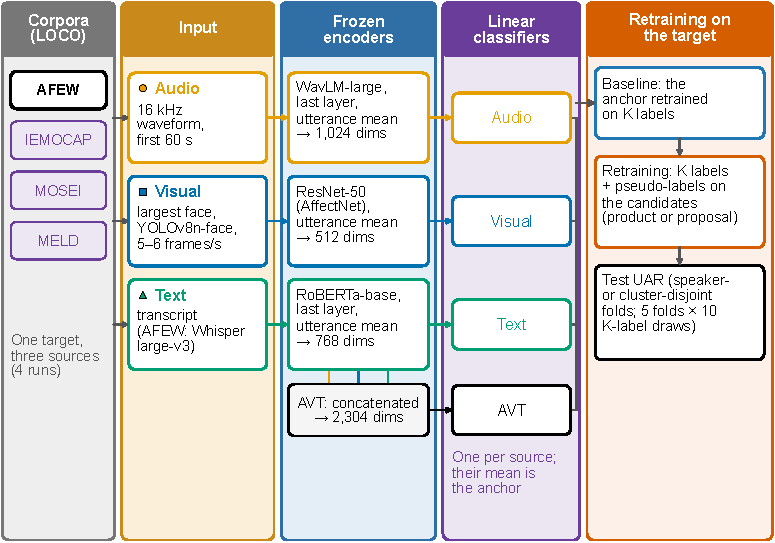
\includegraphics[width=\textwidth]{figures/fig_v4_pipeline_en.pdf}
\caption{Pipeline of the LOCO experiments. One of the four corpora is the target and the other three are the sources (four runs). The audio, visual and text inputs are passed through frozen encoders to give utterance-level features, and the three are also concatenated (AVT). Linear classifiers are trained per source, and the mean of the weights and intercepts of the three source classifiers is the anchor. On the target, the baseline (the anchor retrained on K labels per emotion) and classifiers retrained on the K labels and pseudo-labels on the candidate utterances (the product for the audio, visual, text and AVT classifiers; the proposal for the AVT classifier) are compared on the UAR of test utterances from speaker- or cluster-disjoint folds. AFEW is shown as the target. The evaluation of the proposal with CREMA-D as the target (Sects.~\ref{sec:res-prop}--\ref{sec:res-retrain} and Supplementary Information S7) uses audio and visual only, with four source corpora}\label{fig:pipeline}
\end{figure}

\subsection{Distillation and compared methods}\label{sec:distill}
Distillation retrains each of the audio, visual and text classifiers and the AVT classifier on pseudo-labels. The pseudo-label $q_i$ of each candidate utterance is the \emph{product}: the audio, visual and text classifiers are retrained from the anchor on the K labels and on the probabilities that the baseline AVT classifier assigns to the candidates, and their three probabilities are multiplied per utterance and normalised. $q_i$ includes the prediction of the retrained classifier's own modality. The loss of the retrained linear classifier is the cross-entropy on the K labels plus the cross-entropy towards the pseudo-labels of the candidates (the pseudo-label probabilities are targets without temperature) plus L2 terms towards the anchor $(W_0,b_0)$:
\begin{equation}
\begin{split}
L(W,b)=\frac{1}{S}\Big[&a\sum_{i\in\mathcal{K}}-\log p(y_i\mid x_i)+\sum_{i\in\mathcal{U}}\sum_k g_{ik}\,(-\log p(k\mid x_i))\\
&+\frac{\|W-W_0\|^2}{2C'}+\frac{\|b-b_0\|^2}{2C_b}\Big],
\end{split}
\end{equation}
with $p(\cdot\mid x)=\mathrm{softmax}(Wx+b)$ and $g_{ik}=(\rho n/4)\,q_{ik}/\sum_{j\in\mathcal{U}}q_{jk}$, where $\mathcal{K}$ is the set of K labelled utterances, $\mathcal{U}$ is the set of all $n$ candidates (including $\mathcal{K}$) and $S$ is the sum of the loss weights. The pseudo-label weights sum to $\rho n/4$ for each emotion. This loss form was fixed before the evaluation run; five other loss forms, including the temperature loss of Albanie et al.\ \cite{hinton2015distilling,albanie2018}, are compared in Supplementary Information S4. $C'$ and $C_b$ are those of the baseline; the pseudo-label weight $\rho$, the K-label multiplier $a$ and the exponents of each modality in the product were chosen on the mean UAR over provisional targets (Sect.~\ref{sec:protocol}); when several points were within two standard errors of the best, the one closest to the untuned values ($\rho=1$, $a=1$, exponents (1, 1, 1)) was chosen (grids in Supplementary Information S4). In all 48 conditions with K = 5, 10 and 25, the selected values gave the same classifier as the untuned values, so the product of distillation multiplies the three probabilities with equal weights.

In the LOCO setting, distillation is compared with 11 methods that do not use pseudo-labels including other modalities: self-training \cite{lee2013pseudolabel}, entropy minimisation \cite{grandvalet2004}, IM \cite{liang2020,boudiaf2020}, T3A \cite{iwasawa2021}, label propagation \cite{zhou2004,iscen2019}, a version that uses the retrained classifier's own baseline probabilities as pseudo-labels, training on labelled source utterances and the K labels together (S+T), CORAL \cite{sun2016coral}, DANN \cite{ganin2016dann}, MME \cite{saito2019mme} and an xMUDA-style method \cite{jaritz2020xmuda} (K = 5 UARs in Table~S4; content of each method in the notes of Table~S9). The xMUDA-style method makes unimodal classifiers imitate each other's predictions, so it uses predictions of other modalities but no pseudo-labels including other modalities (computed for the audio, visual and text classifiers only). All methods start from the same anchor and K labels as distillation and select hyperparameters by the same procedure. Because the encoders are frozen, DANN and MME are versions with their loss terms on a linear map and classifier, not the original methods that also train the feature extractor. In the all-source setting, the provider and weighting of the pseudo-labels of distillation were chosen per condition on provisional targets (mostly the product of the classifiers' probabilities), and distillation was compared with eight methods that use same-modality unlabelled utterances (entropy minimisation, self-training, IM, T3A, label propagation, CORAL, DANN and MME). The comparators of the combinations of predictions (Sects.~\ref{sec:res-prop} and \ref{sec:res-ablation}) and of the retrained AVT (Sect.~\ref{sec:res-retrain}) are described in those sections.

\textbf{Retraining with other pseudo-label providers.} In the evaluation run, each of the four classifiers was also retrained on predictions of other classifiers instead of the product, with untuned $\rho=1$ and $a=1$. The providers are classifiers of the baseline (unimodal classifiers of other modalities, classifiers on two concatenated modalities, AVT), the product, the three classifiers that make the product, the AVT anchor and the classifiers of each source corpus. K is 5 and 25, for which the candidate decisions of the baseline were saved. Excluding AVT retrained on its own predictions and duplicates of other providers leaves 360 variants per K (the excluded variants are in Supplementary Information S2; one of them, whose advantage is zero by construction, had a gain interval above zero). For each variant we measure (Fig.~\ref{fig:margintoy}):
\begin{itemize}
\item the \emph{advantage} (the difference in correctness of the pseudo-labels): UAR of the provider's decisions $-$ UAR of the baseline before retraining, on candidates excluding the K labels, using candidate labels that are never used for retraining;
\item the \emph{gain}: UAR of the retrained classifier $-$ UAR of the baseline on test utterances.
\end{itemize}


\begin{figure}[t]
\centering
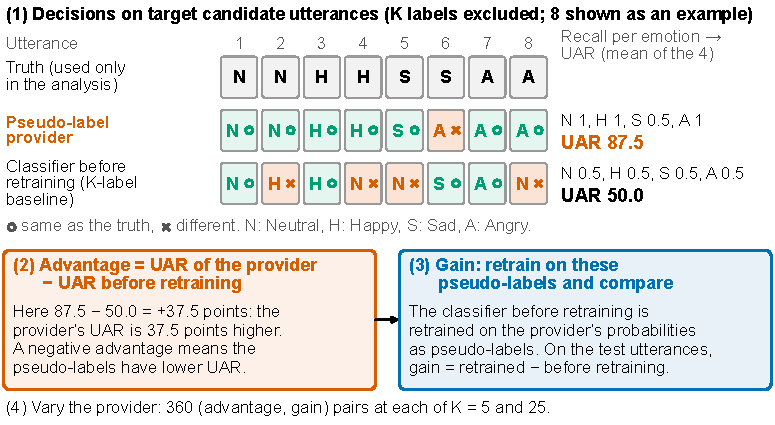
\includegraphics[width=\textwidth]{figures/fig_margin_toy_en.pdf}
\caption{Measuring the advantage and the gain. (1) On the candidate utterances excluding the K labels, the decisions of the pseudo-label provider and those of the classifier before retraining are each scored against the true labels, which are used only for this analysis, giving two UARs. (2) The advantage is the provider's UAR minus the UAR before retraining. (3) The classifier is retrained on the provider's probabilities as pseudo-labels, and the gain is measured on test utterances. (4) Repeating (2) and (3) for each provider gives the (advantage, gain) pairs. The eight utterances and their decisions are illustrative, not experimental values}\label{fig:margintoy}
\end{figure}

\subsection{Measuring the error that remains after removing bias}\label{sec:twoerrors}
A linear classifier assigns an emotion using, for each pair of emotions, a boundary in feature space whose direction is set by the weights and whose position is set by the intercepts (Fig.~S2). An error in which the boundary has the right direction but is shifted, so that predictions are biased towards one emotion, is the \emph{prediction bias}; it disappears when only the intercepts are corrected. The error that remains after correcting the bias is the \emph{remaining error}; it shrinks only when the direction of the weights changes.

We measure the remaining error, for each pair of emotions, as the pairwise accuracy lost because of the boundary direction (the \emph{direction loss}), computed from the distribution of decision values of test utterances relative to the linear discriminant direction of the labelled target utterances (formulas and the fit of the approximation in Supplementary Information S2). Changing only the intercepts, or subtracting each corpus's feature mean, does not change the direction loss. In the all-source setting, we measure whether distillation and each of the eight methods reduce the direction loss, averaged over the six emotion pairs, relative to the baseline. Each condition was classified by pre-set rules as \emph{reduced}, \emph{same level}, \emph{increased} or \emph{undetermined} from the 95\% interval of the direction-loss difference (baseline $-$ method) and an equivalence margin $\delta$ set from provisional-target outputs only (full rules, values of $\delta$ and intervals in Supplementary Information S2). Distillation is measured in 81 conditions (each classifier with audio, visual and text on three corpora and with audio and visual on five corpora; K = 0, 5, 25) and the eight methods in 210 conditions (single modality; K = 0, 5), so the two counts do not compare the same conditions.

\subsection{Proposal: pseudo-labels from per-emotion modality weights}\label{sec:method}

\subsubsection{Idea}\label{sec:idea}
Because distillation retrains classifiers towards pseudo-labels, the goal of the proposal is to raise the UAR of the pseudo-labels' decisions. The product of distillation multiplies the three classifiers' probabilities with equal weights. In computations run to design the method without the evaluation targets (the provisional-target runs of Sect.~\ref{sec:protocol}; each of the four corpora as a provisional target with two of the remaining corpora as sources, 30 repetitions each), the classifier-by-emotion reliabilities (Eq.~\ref{eq:rel} below) measured with all candidate labels were highest for visual on all four emotions of AFEW and for text on all four of MELD, for visual on Happy and audio on the others in IEMOCAP, and changed with the emotion in MOSEI (Fig.~\ref{fig:idea}). We therefore use 12 weights, one per classifier and emotion.

\begin{figure}[t]
\centering
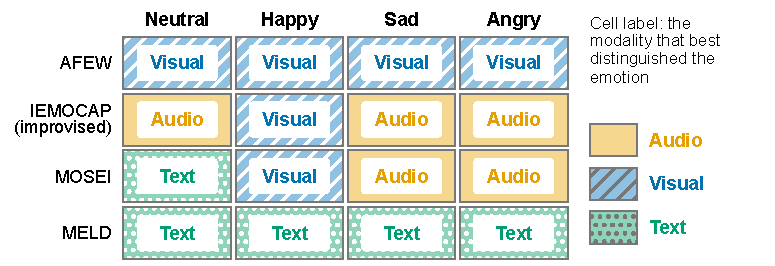
\includegraphics[width=\textwidth]{figures/fig_prop_idea_en.pdf}
\caption{The modality that best separated an emotion differed by corpus and by emotion. Each cell shows the modality with the highest reliability. Values are reliabilities used to design the method (provisional-target computations, all candidate labels, K = 5, mean of 30 repetitions), not values of the evaluation run}\label{fig:idea}
\end{figure}

Measuring all 12 weights on the K target labels would determine each weight from only K utterances per emotion. In the same provisional-target computations, we built two classifier-by-emotion reliability tables, one measured on the sources and one on all candidate labels of the provisional target, and found that splitting the weights into two parts allows each part to be measured on different data (values in Supplementary Information S5). The ranking of classifier strengths (mean reliability over the four emotions) changed across corpora. For every corpus and K, the strongest modality by source-measured strength differed from that on all candidate labels in more than half of the repetitions, and the K-label strengths agreed in more repetitions than the source-measured ones in 11 of the 12 combinations of corpus and K. The classifier-by-emotion component left after removing classifier effects, emotion effects and a non-additivity term, by contrast, correlated positively between the source table and the candidate-label table. We therefore measure strengths on the K target labels and per-emotion profiles on the labelled source corpora. Our goal is not to build a new fusion architecture that learns per-utterance weights, but to set weights that raise the UAR of the pseudo-labels while fitting only three quantities (one strength per classifier) on the K labels.

\subsubsection{Definition}\label{sec:method-def}
The proposal weights the predictions of the classifiers that make the product of distillation (Sect.~\ref{sec:distill}; the product components) with a classifier-by-emotion reliability table and turns the fused predictions into pseudo-labels. The table is the sum of strengths and per-emotion profiles (Fig.~S5). Figure~\ref{fig:propflow} shows how the proposal gives one unlabelled utterance its pseudo-label.

\begin{figure}[t]
\centering
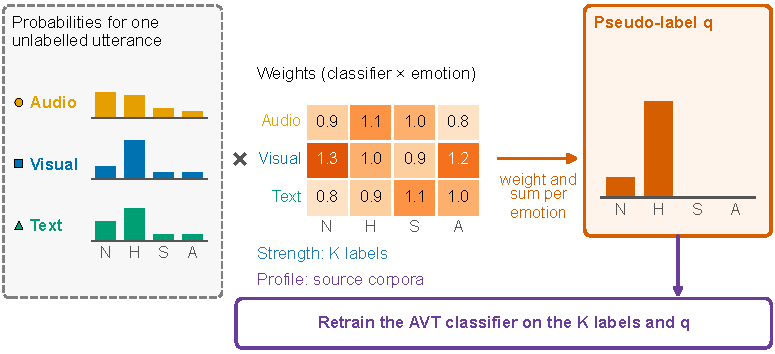
\includegraphics[width=\textwidth]{figures/fig_v4_prop_flow_en.pdf}
\caption{The proposal turns each unlabelled utterance into a pseudo-label q by multiplying the scores (centred log-probabilities) of the three classifiers by classifier-by-emotion weights and summing them per emotion. Left: probabilities that the audio, visual and text classifiers of the product (Sect.~\ref{sec:distill}) assign to one utterance. Middle: the weight table, built from the strengths (measured with classifiers retrained on the K labels without one of five subsets) and the per-emotion profiles (measured on the source corpora) and divided by its mean. Right: q, the softmax of the weighted sum after an intercept shift that uses no labels. The AVT classifier is retrained from the anchor on the K labels and q. Every candidate outside the test set, including the K labelled ones, receives q; test utterances are used only to measure UAR. Probabilities and weights are illustrative; q was computed with the intercept shift set to 0}\label{fig:propflow}
\end{figure}

The reliability is defined on the scores of each classifier. With probabilities $p_m(i\mid x)$ of classifier $m$ for emotion $i$, the centred log-probability is the score $z_m(i\mid x)=\log p_m(i\mid x)-\frac14\sum_j\log p_m(j\mid x)$, and
\begin{equation}\label{eq:rel}
d_m(i)=\max\!\big(0,\sqrt2\,\Phi^{-1}(A_m(i))\big),\quad A_m(i)\in[0.02,0.98],
\end{equation}
where $A_m(i)$ is the mean over emotions $j\neq i$ of the area under the ROC curve (AUC) separating utterances of true emotion $i$ from those of $j$ by $z_m(i\mid\cdot)$, and $\Phi^{-1}$ is the standard normal quantile function ($d_m(i)\le 2.90$). Because the ranks of scores do not change when intercepts are shifted, $d_m(i)$ depends neither on the classifier's intercepts nor on the target's emotion proportions. The mean over the four emotions is the strength $L_m$, and $d_m(i)-L_m$ is the per-emotion profile.

The strengths are measured on the K labels. The K labels are split into five subsets per emotion; for each subset $f$, the product components are retrained by the procedure of distillation on the K labels without subset $f$ and assign probabilities to subset $f$; the reliabilities of Eq.~(\ref{eq:rel}) computed from the five subsets' probabilities are averaged over emotions to give $L^{K}_m$. Because $L^{K}_m$ is noisy for small K, a default strength $L^{0}_m$ (the mean of the three $L^{K}_m$ or the strength measured on the sources) is mixed in with weight $n_0$:
\begin{equation}
L_m=\frac{n\,L^{K}_m+n_0\,L^{0}_m}{n+n_0},\qquad n=4K.
\end{equation}

The profiles are measured on the source corpora. Within each source $s$, $d^{\mathrm{in}}_{s,m}(i)$ is measured by speaker-split five-fold cross-validation, and a classifier trained on all of $s$ is applied to another source $t$ to give $d^{\mathrm{out}}_{s\to t,m}(i)$. The share of modality $m$'s reliability that carries over to other corpora is $\eta_m=\sum_{s\to t}\sum_i d^{\mathrm{out}}_{s\to t,m}(i)/\sum_{s\to t}\sum_i d^{\mathrm{in}}_{s,m}(i)$ (clipped to $[0,1.5]$), and
\begin{equation}
d^{\mathrm{src}}_m(i)=\eta_m\frac{1}{|S|}\sum_s d^{\mathrm{in}}_{s,m}(i),\qquad r^{\mathrm{src}}_m(i)=d^{\mathrm{src}}_m(i)-\frac14\sum_j d^{\mathrm{src}}_m(j)
\end{equation}

The reliability table combines strengths and profiles, and the fused predictions give the pseudo-labels. The table is $T(m,i)=\max(0,L_m+\beta\,r^{\mathrm{src}}_m(i))$ ($\beta=1$ uses the profiles, $\beta=0$ does not); dividing by its mean gives weights $\Omega(m,i)=T(m,i)/(\frac{1}{12}\sum_{m',i'}T(m',i'))$, and the scores are summed per emotion, $s(i\mid x)=\sum_m \Omega(m,i)\,z_m(i\mid x)$. Because emotion-specific weights can shift predictions towards some emotions, intercepts $c$ are shifted without labels so that the mean of $\mathrm{softmax}(s(\cdot\mid x)+c)$ over candidates equals the mean of the product's probabilities (fixed-point iteration). The fused prediction is $\arg\max_i(s(i\mid x)+c_i)$. We attach $q(i\mid x)=\mathrm{softmax}_i(s(i\mid x)+c_i)$ to the candidates as pseudo-labels (soft labels) and retrain the AVT classifier (AV for CREMA-D) with the loss of distillation (Sect.~\ref{sec:distill}). Because the fused predictions carry information of all three modalities, the retrained classifier is AVT, which takes all three features; comparisons of the fused predictions do not depend on this choice. Audio, visual and text classifiers retrained on the proposal's pseudo-labels were not computed (Sect.~\ref{sec:limitations}). $\rho$ and $a$ are borrowed from the values chosen for the product's pseudo-labels.

\subsubsection{Hyperparameters}\label{sec:hp}
The hyperparameters of the proposal ($n_0\in\{0,20,80,\infty\}$, $\beta\in\{0,1\}$ and the two default strengths; 16 settings, 14 distinct) were selected, per evaluation target and K, by the highest mean UAR on the test folds of the provisional targets over three episodes in which each source corpus served in turn as a provisional target with the other two as sources (3 corpora $\times$ 5 folds $\times$ 2 seeds = 30 repetitions; Fig.~S6). No data of the evaluation target enter any episode. All selected settings had $\beta=1$, and $n_0$ was 0 in 8 of 12 conditions and 20 in the other four. The setting $n_0=\infty$, $\beta=0$ with the mean default strength gives the same decisions as the product. For CREMA-D, the hyperparameters ($n_0=0$, $\beta=1$) and $\rho$ and $a$ for the AV classifier were selected on the repetitions of a six-corpus provisional-target computation (the four corpora plus CREMA-D and RAVDESS) that do not involve CREMA-D.

\subsection{Evaluation protocol and intervals}\label{sec:protocol}
LOCO hyperparameters were selected on runs in which each of the three corpora other than the evaluation target served in turn as a provisional target (with the remaining two corpora as sources; 3 corpora $\times$ 5 folds $\times$ 2 seeds = 30 repetitions) and fixed, and the evaluation target was computed once with the fixed settings (the evaluation run). We call each provisional-target computation an \emph{episode}.

The main metric is UAR (unweighted average recall over emotions), whose chance level with four emotions is 25\%. Overall accuracy (weighted accuracy) is not reported because it depends on the share of Neutral, which differs across corpora. UAR and its differences are in percentage points, and the difference A $-$ B between two classifiers is called the \emph{gain}. All intervals are 95\% intervals without multiple-comparison correction; they reflect the sampling of test speakers (clusters for MOSEI and the LOCO setting) and of the K labels, not the choice of source corpora, training utterances, methods or hyperparameters. For the LOCO setting, the variance of a cluster jackknife (cluster resampling for MOSEI and CREMA-D) is added to the variance over K-label draws; because inference with few clusters is anti-conservative \cite{cameron2008}, jackknife $t$ intervals are used for corpora with fewer than 20 effective test clusters. Intervals of the all-source setting are described in Supplementary Information S2. Conditions of the same corpus that differ only in K share test utterances and nested K labels and are not independent. We write that UAR \emph{rose} or \emph{fell} only when the 95\% interval of the difference lies above or below zero, and write ``higher'' or ``lower'' for point estimates.

The order of the work was as follows. The loss form and the hyperparameter grids of distillation were fixed before the evaluation run. The authors inspected UARs and differences (without intervals) of distillation and the 11 methods during the evaluation run (AFEW, IEMOCAP) and before aggregation (four corpora); aggregation scripts and designs were fixed before the evaluation run and not changed afterwards. The idea of the proposal was conceived after seeing outputs of the evaluation run of distillation, its form was fixed after seeing the provisional-target runs, and its evaluation was computed once. CREMA-D was added to the evaluation after its values had been seen in the six-corpus provisional runs. Some pseudo-label options of the all-source setting (such as the product) were added after seeing results of an earlier version of the method on the same corpora. The analysis with other pseudo-label providers (Sect.~\ref{sec:res-margin}) and the comparison with the strongest single classifier (Sect.~\ref{sec:res-prop}) were descriptive analyses set up after the computation from saved outputs, without prior predictions; the former was set up after the gains and intervals of audio, visual and text classifiers retrained on some providers had been seen. Variants share candidates, test utterances and pseudo-label ingredients, so the rank correlations and counts of Sect.~\ref{sec:res-margin} are not tests.

% English version of paper/ja_v4/04_結果.md (ver4, 2026-11-17). Subsection titles state conclusions (MIT CommLab results formula; Mensh & Kording rule 7); each paragraph ends with its answer. Sentences carried over from v3_04_analysis and v3_06_experiments with conditions called by name. Table 2: audio rows of the v3 gain table; Table 3: v3 Table 3(b); Table 4: counts per comparator (full table: Table S10). Figs. 3 and 5: paper/scripts/make_figs_v4.py.
\FloatBarrier
\section{Results}\label{sec:results}

\subsection{Audio classifiers retrained by distillation had higher UAR than the 11 methods that do not use pseudo-labels including other modalities}\label{sec:res-methods}
Table~\ref{tab:audiogain} gives the difference in UAR between audio classifiers retrained by distillation and the baseline. Audio UAR after distillation was higher than that of the baseline in all 12 conditions with four corpora and K = 5, 10 and 25, with intervals above zero in the nine conditions other than IEMOCAP (+2.71 to +4.15\pt). On IEMOCAP, the differences were +1.45 to +2.41\pt, with intervals including zero at all three K. Against the 11 methods that do not use pseudo-labels including other modalities, distillation was higher in all 132 comparisons over the 12 conditions, with intervals not above zero only in 10 comparisons on IEMOCAP (Fig.~\ref{fig:vsmethods}; K = 5 UARs in Table~S4). The version that uses the classifier's own baseline probabilities as pseudo-labels gave $-$1.0 to +0.5\pt\ relative to the baseline. For audio classifiers, pseudo-labels including other modalities gave higher UAR than the 11 methods that do not use them.

\begin{table}[!htbp]
\caption{Audio UAR after distillation was higher than that of the baseline in all 12 conditions with K = 5, 10 and 25, with intervals above zero in the nine other than IEMOCAP. Values: audio classifier retrained by distillation $-$ baseline (UAR points on test utterances) with 95\% intervals without correction, averaged over 50 repetitions (5 for K = 0). At K = 0, the baseline is the anchor (source only) and distillation uses no labels. K = 10 values follow an aggregation decided before the evaluation run (intervals only, no tests). IEMOCAP: improvised part. Visual, text and AVT classifiers: Table~S3}\label{tab:audiogain}
\footnotesize\setlength{\tabcolsep}{3.4pt}
\begin{tabular}{@{}lllll@{}}
\toprule
Corpus & K = 0 & K = 5 & K = 10 & K = 25 \\
\midrule
AFEW & +4.86 [+2.32, +7.40] & +4.15 [+2.56, +5.74] & +3.78 [+2.19, +5.38] & +3.32 [+1.40, +5.25] \\
IEMOCAP & +4.76 [+1.89, +7.63] & +2.41 [$-$0.45, +5.27] & +2.01 [$-$0.57, +4.58] & +1.45 [$-$0.48, +3.37] \\
MOSEI & +2.13 [+1.08, +3.19] & +3.19 [+2.38, +3.99] & +4.11 [+3.20, +5.01] & +3.36 [+2.56, +4.16] \\
MELD & +3.89 [+0.28, +7.51] & +3.12 [+1.18, +5.06] & +2.71 [+0.66, +4.77] & +2.86 [+1.21, +4.51] \\
\botrule
\end{tabular}
\end{table}

\begin{figure}[t]
\centering
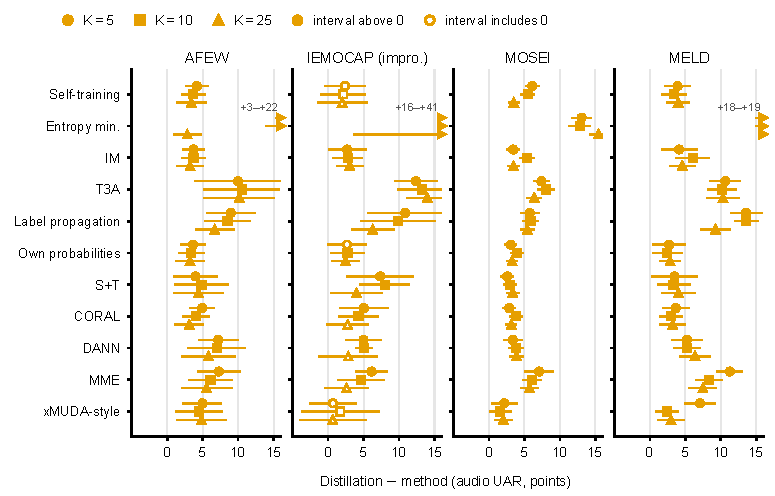
\includegraphics[width=\textwidth]{figures/fig_v4_methods_en.pdf}
\caption{Audio classifiers retrained by distillation had higher UAR than the 11 methods that do not use pseudo-labels including other modalities in all 132 comparisons. Points: distillation $-$ method (UAR points; four corpora $\times$ K = 5, 10, 25); lines: 95\% intervals without correction; open markers: intervals including zero (10 comparisons, all on IEMOCAP). Differences above 16\pt\ are drawn as right-pointing markers at the edge (in place of the K markers), with the method's range rounded to integers}\label{fig:vsmethods}
\end{figure}

Without labels (K = 0), the audio gain of distillation also had intervals above zero on all four corpora (+2.13 to +4.86\pt). The audio classifier retrained on pseudo-labels alone (K = 0) had higher UAR than the baseline with 5 and 10 labels per emotion on all four corpora (e.g.\ 53.4 vs 50.1 and 51.1 on AFEW; all values in Supplementary Information S2; no intervals computed). For audio classifiers, pseudo-labels including other modalities gave higher UAR than 5 or 10 labels per emotion.

By contrast, the gains of the visual, text and AVT classifiers varied across corpora (Table~S3). The gain of the text classifier on IEMOCAP was +5.01 to +7.34\pt, with intervals above zero at all three K, and its intervals included zero on the other corpora; visual intervals were above zero only for MOSEI at K = 10 and 25, and AVT intervals only for MELD at all K and MOSEI at K = 25. For AVT, the differences from the 10 methods other than the xMUDA-style method (which was not computed for AVT) were also mixed: some methods, such as self-training on AFEW (72.1 vs 70.8), were higher than distillation, and at K = 5 only CORAL on MOSEI was higher with the interval of the difference below zero. The 11 methods use information other than pseudo-labels including other modalities, so we read these differences as differences in the information used rather than in the quality of the methods.

\subsection{Pseudo-labels including other modalities reduced the error that remains after removing bias, which same-modality unlabelled utterances rarely did}\label{sec:res-remaining}
Table~\ref{tab:remaining} counts, in the all-source setting, the conditions in which distillation and the eight methods using same-modality unlabelled utterances reduced the remaining error (direction loss) relative to the baseline. Distillation reduced the remaining error in 38 of 81 conditions and increased it in one; its UAR was judged higher than the baseline (same rule) in 32 and lower in none. The eight methods reduced the remaining error in 7 of 210 conditions and increased it in 79. If the true differences were zero and conditions independent, the expected numbers of ``reduced'' conditions would be 2.02 and 5.25. Comparing point estimates on the same anchors and conditions (two modality groups, K = 0 and 5), distillation reduced the remaining error more in 341 of 373 pairs (pairs are not independent). In the all-source setting, the remaining error was reduced mainly by pseudo-labels including other modalities and rarely by same-modality unlabelled utterances.

\begin{table}[!htbp]
\caption{In the all-source setting, the remaining error (direction loss) was reduced in 38 of 81 conditions by distillation and in 7 of 210 by the eight methods using same-modality unlabelled utterances. Values: numbers of conditions by verdict. Direction loss: reduced / same level / increased / undetermined; UAR (method $-$ baseline): higher / same level / lower / undetermined. ``16 more'' are conditions in which the adaptation term of DANN or MME did not change predictions beyond seed variation (separate from the 48 undetermined). Visual direction losses come from features that failed the approximation check (Supplementary Information S2)}\label{tab:remaining}
\footnotesize
\begin{tabular}{@{}lllrll@{}}
\toprule
Method & Modalities & Classifier & Conditions & Direction loss$^{a}$ & UAR \\
\midrule
Distillation & A, V, T (3 corpora) & Audio & 9 & 9/0/0/0 & 9/0/0/0 \\
 &  & Visual & 9 & 1/1/0/7 & 1/0/0/8 \\
 &  & Text & 9 & 5/0/1/3 & 4/0/0/5 \\
 &  & AVT & 9 & 6/1/0/2 & 5/2/0/2 \\
 & A, V (5 corpora) & Audio & 15 & 7/0/0/8 & 7/0/0/8 \\
 &  & Visual & 15 & 5/0/0/10 & 4/1/0/10 \\
 &  & AV & 15 & 5/5/0/5 & 2/2/0/11 \\
\midrule
Distillation, total & & & 81 & 38/7/1/35 & 32/5/0/44 \\
Eight methods & Single modality & A, V, T & 210 & 7/60/79/48 (16 more) & --- \\
\botrule
\end{tabular}
\footnotetext{$^{a}$Halving $\delta$ gives 49 of 81 ``reduced'' conditions for distillation; doubling it gives 20}
\end{table}

\subsection{The more accurate the pseudo-labels were than the classifier before retraining, the higher the UAR after retraining}\label{sec:res-margin}
We related the advantage to the gain over the variants retrained with other pseudo-label providers (Sect.~\ref{sec:distill}). For example, on MOSEI with K = 25, retraining the audio classifier on pseudo-labels from the visual--text classifier gave an advantage of +4.6\pt\ (42.2 vs 37.6) and a gain of +2.05 [+0.74, +3.35]\pt. On AFEW with K = 5, retraining the visual classifier on pseudo-labels from the audio--text classifier gave an advantage of $-$16.7\pt\ (54.4 vs 71.1) and a gain of $-$4.40 [$-$7.70, $-$1.09]\pt.

Over the 360 variants, the ranks of advantage and gain agreed: the rank correlation was 0.80 at K = 5 and 0.83 at K = 25, and within each of the 32 combinations of corpus, retrained classifier and K it was positive (median 0.92, minimum 0.39). Figure~\ref{fig:margincounts} counts the variants by the sign of the advantage and the gain interval. No variant with a negative advantage (173 at K = 5, 184 at K = 25) had a gain interval above zero, and 125 and 144 had intervals below zero. Among variants with a positive advantage (187 and 176), 58 and 42 had intervals above zero, while 16 and 20 had intervals below zero (breakdown in Supplementary Information S2). Of the 360 variants counted, every variant whose UAR rose had pseudo-labels more accurate than the classifier before retraining (the one excluded variant whose advantage is zero by construction rose; Supplementary Information S2).

\begin{figure}[t]
\centering
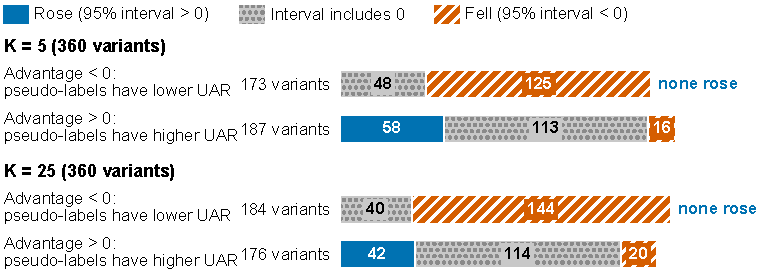
\includegraphics[width=\textwidth]{figures/fig_margin_counts_en.pdf}
\caption{No variant whose pseudo-labels were less accurate than the classifier before retraining (negative advantage) rose (gain interval above zero). Variants retrained with other pseudo-label providers (360 per K; K = 5 and 25) counted by the sign of the advantage and by the 95\% interval of the gain (above zero, including zero, below zero). One variant is one combination of corpus, retrained classifier and pseudo-label provider; the gain is the difference in test UAR}\label{fig:margincounts}
\end{figure}

Among unimodal classifiers, the one whose baseline had the highest candidate UAR (hereafter the corpus's strongest modality) was visual on AFEW, audio on IEMOCAP, visual on MOSEI and text on MELD at both K = 5 and 25. Retraining the classifier of the strongest modality on pseudo-labels from the classifier on the concatenated features of the other two modalities gave negative gains in point estimates in all eight cases (four corpora and two K; $-$4.40 to $-$1.02\pt). The classifier of the strongest modality had lower UAR than before retraining, in point estimates, when it was retrained on pseudo-labels from the other two modalities alone.

\subsection{Predictions fused by the proposal had higher UAR than the equal-weight product in 11 of 12 conditions}\label{sec:res-prop}
Figure~\ref{fig:propfig}(a) shows the difference in UAR between the proposal and the product, and Table~\ref{tab:propcount} counts, for each way of combining the three classifiers' predictions, the signs and intervals of the differences from the proposal (UARs and differences in Table~S10). The fused predictions are the argmax of the combined predictions of the three classifiers on test utterances, without retraining any classifier. Proposal $-$ product was positive in 11 of 12 conditions, with 95\% intervals excluding zero in seven (AFEW at all K, IEMOCAP and MOSEI at K = 25, MELD at K = 10 and 25). The largest differences were on AFEW (+2.13 to +3.51\pt). On AFEW, the visual product component's UAR exceeded the audio and text components by more than 17\pt\ (K = 5: visual 70.70, audio 53.24, text 45.76), and the visual classifier alone was higher than the product at K = 5 and 10 (70.70 vs 69.23, 71.93 vs 70.88). On IEMOCAP, MOSEI and MELD, proposal $-$ product ranged from $-$0.09 to +0.83\pt\ over the nine conditions. The difference from the probability mean was positive in 8 of 12 conditions, with intervals above zero on AFEW at all K and MOSEI at K = 25 and none below zero. The proposal made more accurate predictions than the equal-weight product in 11 of 12 conditions and than the probability mean in 8.

\begin{table}[!htbp]
\caption{The proposal had higher UAR than every comparator in at least 8 of 12 conditions; intervals lay below zero (proposal lower) in only one condition against temperature calibration and two against the version without strength differences. Values: counts over 4 corpora $\times$ K = 5, 10, 25 of the difference proposal $-$ comparator (for retrained AVT: AVT retrained on the proposal's pseudo-labels $-$ comparator), with 95\% intervals without correction. The strongest single classifier was added after the evaluation run (Sect.~\ref{sec:protocol}). UARs and differences per condition: Table~S10; CREMA-D (audio and visual): Table~S8}\label{tab:propcount}
\footnotesize
\begin{tabular}{@{}p{4.5cm}cccl@{}}
\toprule
Comparator & Positive & Interval above 0 & Interval below 0 & Range (points) \\
\midrule
\multicolumn{5}{@{}l}{\textit{Fused predictions}} \\
Product (equal weights) & 11 & 7 & 0 & $-$0.09 to +3.51 \\
Probability mean & 8 & 4 & 0 & $-$0.49 to +3.73 \\
Per-classifier temperature calibration & 8 & 4 & 1 & $-$2.94 to +1.18 \\
Strongest single classifier on the K labels & 12 & 7 & 0 & +2.70 to +5.52 \\
Proposal without per-emotion profiles & 12 & 5 & 0 & +0.10 to +0.73 \\
Proposal without strength differences & 8 & 3 & 2 & $-$0.42 to +3.20 \\
\multicolumn{5}{@{}l}{\textit{Retrained AVT}} \\
Baseline AVT & 10 & 7 & 0 & $-$0.56 to +3.05 \\
AVT retrained on the product's pseudo-labels & 11 & 5 & 0 & $-$0.05 to +1.95 \\
\botrule
\end{tabular}
\end{table}

\begin{figure}[t]
\centering
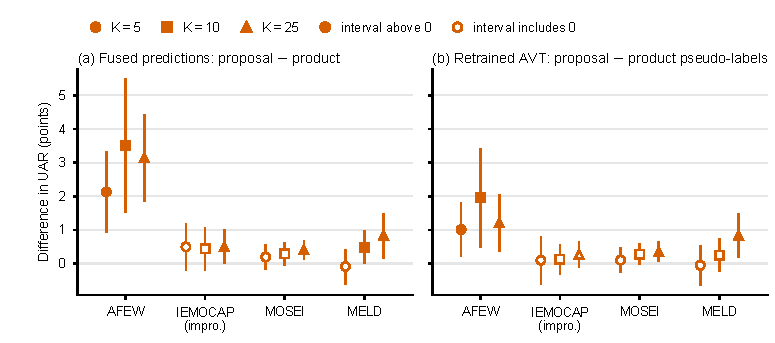
\includegraphics[width=\textwidth]{figures/fig_v4_prop_en.pdf}
\caption{Predictions fused by the proposal had higher UAR than the equal-weight product, and AVT classifiers retrained on the proposal's pseudo-labels had higher UAR than those retrained on the product's pseudo-labels, each in 11 of 12 conditions, with the largest differences on AFEW. (a) Fused predictions: proposal $-$ product. (b) AVT retrained on the proposal's pseudo-labels $-$ AVT retrained on the product's pseudo-labels. Points: differences; lines: 95\% intervals without correction; open markers: intervals including zero}\label{fig:propfig}
\end{figure}

By contrast, differences from comparators that fit to the few labels or select one classifier depended on the comparator. Against per-classifier temperature calibration (inverse temperatures fitted to the K-label log-likelihood \cite{guo2017calibration}; three quantities fitted on the K labels, as in the proposal), the difference was positive in 8 of 12 conditions, and the proposal was lower with the interval excluding zero only on AFEW at K = 5 ($-$2.94 [$-$5.6, $-$0.3], 71.36 vs 74.30). Against the single classifier with the highest K-label strength, the proposal was higher in all 12 conditions (+2.70 to +5.52\pt), with intervals above zero in seven (IEMOCAP at K = 5, MOSEI and MELD at all K). Decomposing the difference, multiplying the three classifiers' predictions (product $-$ strongest single: +2.04 to +5.02\pt) accounted for most of it on IEMOCAP, MOSEI and MELD, and changing the weights (proposal $-$ product) accounted for most of it on AFEW (details in Supplementary Information S5). Comparisons with seven further combinations are in Supplementary Information S6.

\subsection{Removing strength differences lowered UAR on AFEW, and removing per-emotion profiles lowered UAR on MOSEI}\label{sec:res-ablation}
We compared the proposal with versions without one of its parts (Table~\ref{tab:propcount}; Table~S10). On MOSEI, the difference from the proposal without per-emotion profiles had intervals above zero at all K (+0.51 to +0.73\pt), and so did CREMA-D (Supplementary Information S7). On AFEW, the difference from the proposal without strength differences had intervals above zero at all K (+1.74 to +3.20\pt), accounting for most of AFEW's proposal $-$ product (+2.13 to +3.51\pt). On MOSEI at K = 5 and 10, by contrast, the version without strength differences had higher UAR ($-$0.42 [$-$0.7, $-$0.1] and $-$0.35 [$-$0.6, $-$0.1]\pt). Counted after the evaluation over its 50 repetitions, the classifier with the highest K-label strength was the classifier with the highest strength on all candidate labels (visual on AFEW, audio on IEMOCAP, text on MELD) in 0.70--1.00 of repetitions, whereas the classifier with the highest source-measured strength was a different classifier on all three corpora. On MOSEI, where the top two strengths were close, this fraction was 0.30--0.38 (values per corpus and K in Supplementary Information S5). Strength differences raised the proposal's UAR on AFEW, where the visual classifier's UAR exceeded those of the audio and text classifiers by more than 17\pt, and per-emotion profiles raised it on MOSEI, where the strongest modality changed with the emotion.

\subsection{AVT classifiers retrained on the proposal's pseudo-labels also had higher UAR than those retrained on the product's pseudo-labels in 11 of 12 conditions}\label{sec:res-retrain}
We retrained the AVT classifier on the proposal's pseudo-labels (Fig.~\ref{fig:propfig}(b); lower part of Table~\ref{tab:propcount}). Its UAR was higher than that of the AVT retrained on the product's pseudo-labels in 11 of 12 conditions, with intervals above zero in five (AFEW at all K, MOSEI and MELD at K = 25; +1.01, +1.95 and +1.21\pt\ on AFEW); the other nine differences ranged from $-$0.05 to +0.82\pt. Against the baseline AVT, the difference was positive in 10 of 12 conditions and above zero in seven. On CREMA-D (audio and visual), proposal $-$ product of the fused predictions and AV retrained on the proposal's pseudo-labels $-$ AV retrained on the product's pseudo-labels were +0.31 to +0.63\pt, with all six intervals excluding zero (Supplementary Information S7). Classifiers retrained on the proposal's pseudo-labels, whose fused predictions were more accurate than the product, also had higher UAR than those retrained on the product's pseudo-labels.

% English version of paper/ja_v4/05_考察.md (ver4, 2026-11-17). MIT CommLab discussion: main conclusion -> answers to the questions of the introduction -> agreement and disagreement with prior work -> what the limitations leave open -> next steps. Cited claims as in reviews/v4_ja/citations_2026-11-17.md.
\FloatBarrier
\section{Discussion}\label{sec:discussion}

The main conclusion of this study is that, on a new corpus with few labels, the other modalities of the same utterance made up for part of the missing labels, and how much they made up depended on how the pseudo-labels were built. Albanie et al.\ \cite{albanie2018} and Zhang et al.\ \cite{zhang2021combining} showed that classifiers can be trained on predictions of other modalities; we showed, by comparison under the same conditions in a cross-corpus setting with only a few target labels, that doing so gave audio classifiers higher UAR than domain adaptation, semi-supervised and test-time adaptation methods.

The answers to the two questions of the introduction are as follows. First, on whether same-modality methods using unlabelled utterances or pseudo-labels including other modalities make better classifiers, pseudo-labels including other modalities gave audio classifiers higher UAR (Sect.~\ref{sec:res-methods}). In the all-source setting, same-modality unlabelled utterances rarely reduced the remaining error, whereas pseudo-labels including other modalities reduced it in nearly half of the conditions (Sect.~\ref{sec:res-remaining}). One possible explanation is that same-modality unlabelled utterances add only information on the distribution of features the classifier already uses, whereas predictions of other modalities add separate cues about the emotion of the utterance. Another possible explanation of why distillation gave audio classifiers gains with intervals above zero in 9 of 12 conditions is that audio features predicted the decisions of the text classifier, which is part of the product, better than visual features did (Supplementary Information S3; its relation to the gains was not measured). Second, on how to build the pseudo-labels, retrained classifiers had higher UAR the more accurate the pseudo-labels were relative to the classifier before retraining (Sect.~\ref{sec:res-margin}), and setting per-emotion weights of each modality from the few labels and the sources produced pseudo-labels more accurate than equal weights, with higher UAR also for classifiers retrained on them (Sects.~\ref{sec:res-prop}--\ref{sec:res-retrain}).

Our results agree and disagree with prior work in the following points. That distillation gave audio classifiers higher UAR is in the same direction as Albanie et al.\ \cite{albanie2018}, who showed that audio emotion classifiers can be trained on facial predictions; we confirmed it in a cross-corpus setting with only a few target labels. Training on the predictions of a more accurate model of another modality has been reported not to always improve the trained model \cite{xue2023mfh}. In our results, no variant with a negative advantage, that is, with pseudo-labels less accurate than the classifier before retraining, rose, and UAR rose for only some variants with more accurate pseudo-labels (Sect.~\ref{sec:res-margin}). This suggests that pseudo-labels being no less accurate than the classifier before retraining is a necessary, but not a sufficient, condition for UAR to rise. The emotion-dependent differences in modality strength that Busso et al.\ \cite{busso2004} reported within one corpus were also observed across our corpora, where the ranking of classifier strengths changed from corpus to corpus (Sect.~\ref{sec:idea}). Saito et al.\ \cite{saito2019mme} reported that, when the target has a few labels, unsupervised domain adaptation methods that align feature distributions often do not improve performance relative to just training on labelled source and target examples. In our all-source setting, the eight methods, including versions of DANN and MME moved to linear classifiers on frozen features, rarely reduced the remaining error (Sect.~\ref{sec:res-remaining}). With few training samples, a model trained on more modalities has also been argued to be able to fall below a model trained on a subset of them \cite{huang2021}. The proposal combines the decisions of three separately trained classifiers with three quantities set on the K labels, and it had higher UAR than the single classifier strongest on the K labels in all 12 conditions (Sect.~\ref{sec:res-prop}).

Several points remain open within the scope of this study (Sect.~\ref{sec:limitations}). The classifiers are linear classifiers on frozen encoders, and whether the comparisons give the same results with fine-tuned encoders is unknown. Distillation gave audio classifiers gains with intervals above zero in 9 of 12 conditions, whereas the gains of the visual, text and AVT classifiers varied across corpora. The proposal was built on the same four corpora used to evaluate it, so differences from the product and other combinations may be biased in its favour. The relation between the accuracy of the pseudo-labels and UAR is a descriptive analysis set up after the computation.

We plan three next steps. First, we will compare same-modality methods with pseudo-labels from other modalities using fine-tuned encoders and other corpora. Second, we will evaluate the proposal once on a new corpus with the procedure fixed and retrain the audio, visual and text classifiers on its pseudo-labels. Third, we will estimate from the few labels whether the pseudo-labels are more accurate than the classifier before retraining, and turn this into a procedure for choosing pseudo-label providers. Building MER classifiers for a new corpus involves weighing the effort of labelling against that of collecting unlabelled multimodal recordings; as material for this decision, our results showed how much pseudo-labels including other modalities made up for the shortage of labels and that this depended on how the pseudo-labels were built.

% English version of paper/ja_v4/06_限界.md (ver4, 2026-11-17): five paragraphs; the answer-bias paragraph moved to Supplementary Information S2. Wording carried over from v3_08_limitations.tex.
\section{Limitations}\label{sec:limitations}

This study has five limitations.

\textbf{Settings, corpora and encoders.} Section~\ref{sec:res-remaining} uses the all-source setting, and Sects.~\ref{sec:res-methods} and \ref{sec:res-margin}--\ref{sec:res-retrain} the LOCO setting. IEMOCAP in the LOCO setting is only its improvised part, and all corpora are in English. One frozen encoder per modality was used. Fine-tuned audio encoders have been reported to give better dimensional emotion prediction (CCC, the concordance correlation coefficient) than frozen features \cite{wagner2023}, so whether the gains of distillation or the reduction of the error are the same with fine-tuning is unknown. For visual features, the median approximation error of the direction loss was 0.47 times the median direction loss, failing the pre-set criterion (below 1/3; Supplementary Information S2), so the visual rows of Table~\ref{tab:remaining} should be read as values that include errors of the same size as the approximation. The values should be read as values for four or five English corpora and linear classifiers on one frozen encoder per modality. Checking other corpora and fine-tuned encoders is the next step.

\textbf{Analyses and methods built on the same data.} The analysis with other pseudo-label providers (Sect.~\ref{sec:res-margin}) and the comparison with the strongest single classifier (Sect.~\ref{sec:res-prop}) were set up after the computation from saved outputs, without prior predictions. The forms, grids and selection procedures of distillation and the proposal were built and inspected on the evaluation corpora as described in Sect.~\ref{sec:protocol}, and the test folds of each corpus also served as provisional-target tests for other targets. Differences from the product and other combinations may therefore be biased in favour of the proposal. Evaluating once on a new corpus with the procedure fixed is the next step.

\textbf{Retrained classifiers and the classifier's own modality in the pseudo-labels.} Only AVT (AV for CREMA-D) was retrained on the proposal's pseudo-labels, not the audio classifier, for which distillation gave positive gains on all four corpora. The pseudo-labels of distillation also include the retrained classifier's own modality, so the gains cannot be attributed to the other modalities alone. The effect of the proposal should therefore be read as values for the fused predictions and retrained AVT. Retraining the audio, visual and text classifiers on the proposal's pseudo-labels, and on pseudo-labels without the classifier's own modality, is the next step.

\textbf{Shared content.} Speakers are separated, but the same person (MOSEI), episode (MELD) or storyline (IEMOCAP) may appear on both sides, and in CREMA-D the same 12 sentences appear on both sides. How much agreement from shared content enters UAR is therefore unknown, and CREMA-D values in particular should be read as values with the same sentences on both sides. Repeating the comparisons with splits that also separate sentences and episodes is the next step.

\textbf{Estimating the advantage, and intervals.} The advantage was measured with all candidate labels, which a new corpus lacks, and only at K = 5 and 25. Section~\ref{sec:res-margin} therefore describes the variants whose UAR rose rather than giving a procedure for choosing pseudo-label providers. Intervals are not corrected for multiple comparisons, and counts of conditions are not tests. Estimating the advantage within the K labels and comparing it with the value measured on all candidate labels is the next step.

% English version of paper/ja_v4/07_結論.md (ver4, 2026-11-17): one paragraph, no numbers repeated from the abstract (MIT CommLab, Widom), ending with how the pseudo-labels are built; last sentence made positive on 2026-11-17 night (researcher's comment), with the comparator stated (reviews/v4_ja/numbers_intro_rq_2026-11-17.md, item 12).
\section{Conclusion}\label{sec:conclusion}

For multimodal emotion recognition on a new corpus with only a few labels per emotion, we compared distillation on pseudo-labels including other modalities with domain adaptation, semi-supervised and test-time adaptation methods that do not use such pseudo-labels, under the same conditions, with linear classifiers on frozen encoders. For audio classifiers, retraining on pseudo-labels including other modalities gave higher UAR than the compared methods, and, across pseudo-labels from different providers, retrained classifiers had higher UAR the more accurate the pseudo-labels were than the classifier before retraining. In the all-source setting, same-modality unlabelled utterances rarely reduced the remaining error (the error left after correcting prediction bias). In addition, to make the pseudo-labels more accurate, we proposed late fusion that sets the weights of each modality's predictions with strengths from the few target labels and per-emotion profiles from the source corpora. The proposal produced more accurate pseudo-labels than equal-weight fusion. On a new corpus with few labels, the other modalities of the same utterance made up for part of the missing labels, and weighting the modalities with the few target labels and the source corpora, rather than equally, gave AVT classifiers retrained on the resulting pseudo-labels higher UAR in most conditions.


\backmatter

\bmhead{Acknowledgements}
TODO

\section*{Declarations}

\begin{itemize}
\item \textbf{Funding:} TODO (mandatory; state explicitly if none).
\item \textbf{Competing interests:} The authors declare no competing interests. TODO (confirm)
\item \textbf{Ethics approval and consent to participate:} This study is a secondary analysis of research corpora distributed for research (IEMOCAP, CMU-MOSEI, MELD, AFEW, CREMA-D, RAVDESS); no new data were collected from people. TODO (state the providers' approvals and consent as documented by each corpus)
\item \textbf{Consent for publication:} Not applicable.
\item \textbf{Data availability:} The corpora are available from their distributors \cite{busso2008iemocap,zadeh2018mosei,poria2019meld,dhall2012afew,cao2014cremad,livingstone2018ravdess}; IEMOCAP and AFEW are distributed under licence agreements. Utterance lists, label mappings and splits will be released at TODO. Transcripts of AFEW and of reversed speech are not released because they contain licensed corpus content; the scripts and Whisper settings used to produce them are released with the code.
\item \textbf{Code availability:} The code, the utterance identifiers, the splits and the scripts that produce all tables and figures are available at \url{https://github.com/snics6/mer-crosscorpus-pseudolabels} under the MIT licence (version DOI: TODO); software versions and hardware are listed in the repository.
\item \textbf{Author contribution:} TODO (CRediT roles).
\item \textbf{Supplementary information:} Supplementary Information (Online Resource 1, file ESM\_1.pdf) accompanies this article: S1, per-emotion LOCO counts and the settings figure; S2, details of the analysis (error formulas and fit, single-source analysis, verdict rules, excluded variants, per-classifier gains, the 11-method table); S3, predictability of the text classifier's decisions from audio features; S4, details of the distillation loss; S5, method details and the comparator table; S6, further comparisons; S7, CREMA-D results; S8, codes of the compared conditions; S9, the full evaluation table of the proposal.
\item \textbf{Use of generative AI:} An AI assistant (Claude, Anthropic) was used to check the English translation.
\end{itemize}



\bibliography{references}

\end{document}
